\documentclass[conference,a4paper]{IEEEtran}
\IEEEoverridecommandlockouts

\usepackage{cite}
\usepackage{amsmath,amssymb,amsfonts}
\usepackage{algorithmic}
\usepackage{graphicx}
\usepackage{textcomp}
\usepackage{xcolor}
\usepackage{booktabs}
\usepackage{multirow}
\usepackage{url}
\def\BibTeX{{\rm B\kern-.05em{\sc i\kern-.025em b}\kern-.08em
    T\kern-.1667em\lower.7ex\hbox{E}\kern-.125emX}}

\begin{document}

\title{Design-Based KPI Estimation and Survey-Weighted Machine Learning for Undiagnosed Diabetes Screening on NHANES 2017--2018}

\author{\IEEEauthorblockN{Varun Mundhada}
\IEEEauthorblockA{\textit{Department of Computer Science and Engineering} \\
\textit{Symbiosis Institute of Technology, Nagpur}\\
Symbiosis International (Deemed University), Pune, India \\
PRN: 23070521184}
}

\maketitle

\begin{abstract}
Disease that has never been diagnosed is missing from claims, registries and hospital records, so performance indicators built from those sources cannot show it. This work uses the US National Health and Nutrition Examination Survey 2017 to 2018, which interviews and physically examines a national probability sample of 9,254 people, for two purposes. First, a pipeline produces 612 survey-weighted estimates for 17 indicators across utilisation, chronic disease and access, using Taylor-linearised standard errors with 15 design degrees of freedom, logit confidence intervals, statistical suppression, an income concentration index and direct age standardisation, and feeds a three-tier Streamlit dashboard. Among adults with glycated haemoglobin of 6.5 percent or more, 18.0 percent (95 percent CI 14.8 to 21.7) had never been told they had diabetes, about 4.2 million people. Lack of insurance was strongly concentrated among poorer adults (concentration index minus 0.42), but undiagnosed diabetes was not (minus 0.01). Second, logistic regression, random forest, gradient boosting and a multilayer perceptron were trained on 18 non-laboratory features to find undiagnosed diabetes among 4,051 adults, with survey weights and nested cross-validation, and compared with an adapted American Diabetes Association risk score and seven published models. Logistic regression reached a weighted AUC of 0.788 (0.732 to 0.841) against 0.734 for the risk score, a gain that was not statistically significant with 150 cases.
\end{abstract}

\begin{IEEEkeywords}
NHANES, undiagnosed diabetes, complex survey design, concentration index, machine learning, public health dashboard
\end{IEEEkeywords}

\section{Introduction}
Most health performance indicators are built from records that start with a clinical encounter: claims, discharge abstracts, registries and notifiable-disease reports. A person whose diabetes or hypertension has never been detected does not appear in any of them. The US National Health and Nutrition Examination Survey (NHANES) is different because it interviews a national probability sample at home and then measures the same people in a mobile examination centre (MEC). It can therefore count disease that the health system has not yet seen. National estimates put the undiagnosed share of US diabetes between one fifth and one quarter \cite{wang2021,fang2022,gwira2024}.

This project had two aims: to turn NHANES 2017--2018 into a three-tier key performance indicator (KPI) dashboard in which every number is a design-based estimate with a valid interval, and to test whether non-laboratory information is enough to find people with undiagnosed diabetes. The contributions are (i) a reproducible pipeline producing 612 survey-weighted estimates with Taylor-linearised errors, $t$-based intervals and NCHS suppression; (ii) an income concentration analysis with a tie correction, pooled and within age bands; (iii) a nested, survey-weighted comparison of four machine-learning (ML) models with an adapted American Diabetes Association (ADA) risk score and seven published benchmarks; and (iv) a Streamlit dashboard that only reads the audited estimates.

\section{Related Work}
\subsubsection*{Undiagnosed diabetes and hypertension in NHANES} Wang \textit{et al.} found that 23.3\% of US diabetes was undiagnosed in 2017--2018 \cite{wang2021}. Fang \textit{et al.} showed that this share depends on whether a confirmatory second test is required \cite{fang2022}, and studied control trends and screening eligibility \cite{fang2021}; later work extends the series to 2021--2023 \cite{gwira2024,cdc_ndsr}. For blood pressure, control declined after 2013--2014 \cite{muntner2020,muntner2022}, and later cycles report awareness and control \cite{ostchega2020,fryar2024}. Hales \textit{et al.} give the reference obesity estimate \cite{hales2020}.

\subsubsection*{Machine learning for undiagnosed diabetes} De Silva \textit{et al.} found that logistic regression (LR), random forest (RF) and neural networks did not significantly beat the ADA risk test \cite{bang2009} for undiagnosed diabetes in NHANES \cite{desilva2021}; Choi \textit{et al.} found tree ensembles ahead of Korean risk scores \cite{choi2023}. Other NHANES studies report AUCs from 0.75 to 0.91 for outcomes from fasting-glucose to self-reported diabetes \cite{qin2022,riverosperez2025,liu2025,yang2026,yoo2026}, but none of the full texts we checked used the survey weights, which change both the fitted model and its estimated performance \cite{macnell2023,kim2026}.

\subsubsection*{Inequality measurement and dashboards} The concentration index measures how a health variable is distributed across income ranks; Erreygers corrected it for bounded outcomes \cite{erreygers2009}, and recent work applies it along the care cascade \cite{vu2026,okova2026}. Dashboard reviews call for actionable indicators with stated uncertainty \cite{ivankovic2021,schulze2023}. Public NHANES has no geography, so maps need model-based products such as CDC PLACES \cite{greenlund2022}.

\section{Data and Methodology}
\begin{figure*}[t]
\centering
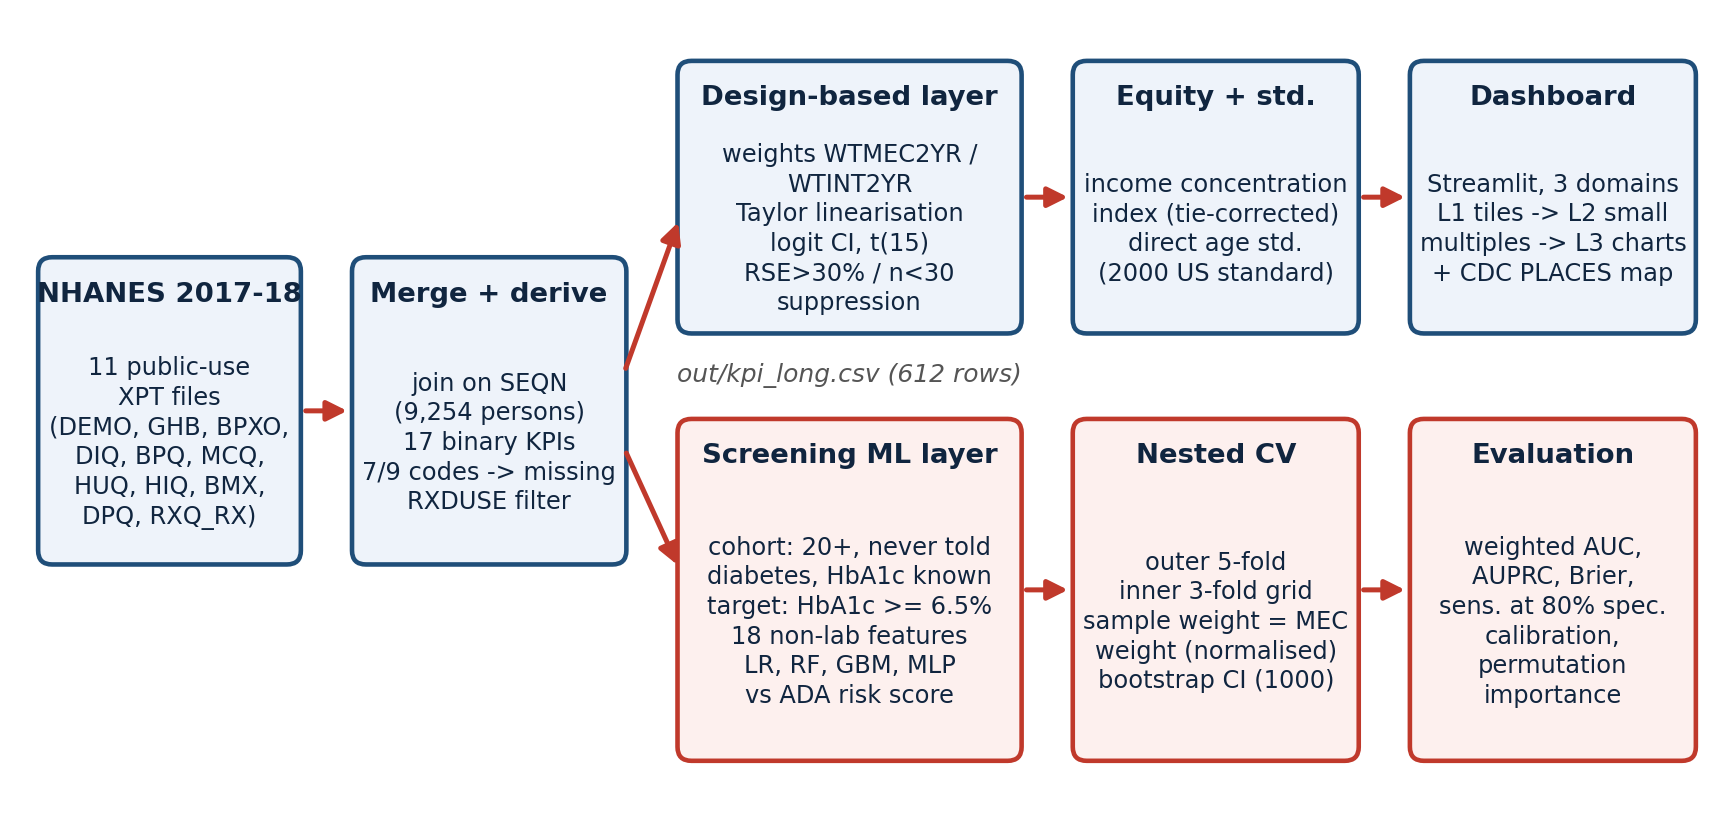
\includegraphics[width=0.66\textwidth]{figures/architecture.png}
\caption{System architecture. The upper path produces the design-based KPI estimates read by the dashboard; the lower path trains and evaluates the screening models on the same analytic file.}
\label{fig:arch}
\end{figure*}
\subsection{Data}
We used 11 public-use NHANES 2017--2018 files: demographics (DEMO), glycohaemoglobin (GHB), oscillometric blood pressure (BPXO), body measures (BMX), the diabetes (DIQ), blood-pressure (BPQ), medical-conditions (MCQ), utilisation (HUQ), insurance (HIQ) and PHQ-9 depression (DPQ) questionnaires, and prescription medicines (RXQ\_RX). Files were merged on the respondent identifier SEQN, giving 9,254 persons with no duplicates. Codes 7 and 9 (refused, don't know) were set to missing, and prescription counts used only rows with \texttt{RXDUSE}$=1$.

\subsection{Indicators}
Seventeen binary indicators were defined for adults aged 18 and over, grouped into three domains. \textit{Utilisation and patient experience}: fair or poor self-rated health, overnight admission in the past 12 months, four or more care contacts, having a usual source of care, and the emergency department as usual source. \textit{Chronic disease}: HbA1c $\geq$6.5\% (laboratory diabetes), self-reported diagnosis, any diabetes, undiagnosed diabetes (laboratory-positive and never told, among the laboratory-positive), prediabetes (HbA1c 5.7--6.4\%), measured hypertension at 130/80 and 140/90 mmHg (mean of up to three readings), undiagnosed hypertension at each threshold, obesity (BMI $\geq$30) and depression (PHQ-9 $\geq$10). \textit{Access}: uninsured and polypharmacy ($\geq$5 prescriptions). Respondents who answered ``borderline'' to the diabetes question were treated as diagnosed in the primary analysis and as undiagnosed in a sensitivity analysis.

\subsection{Design-based estimation}
NHANES is a stratified, multistage cluster sample, so estimates use the MEC weight $w_i$ (\texttt{WTMEC2YR}) for examination or laboratory indicators and the interview weight (\texttt{WTINT2YR}) otherwise. A prevalence is the ratio estimator
\begin{equation}
\hat p = \frac{\sum_i w_i y_i}{\sum_i w_i},
\end{equation}
and its variance is obtained by Taylor linearisation with a with-replacement approximation over strata $h$ and primary sampling units (PSUs) $j$:
\begin{equation}
\widehat{\mathrm{Var}}(\hat p) = \frac{1}{\left(\sum_i w_i\right)^2}\sum_{h}\frac{n_h}{n_h-1}\sum_{j=1}^{n_h}\left(z_{hj}-\bar z_h\right)^2,
\end{equation}
where $z_{hj}=\sum_{i\in(h,j)} w_i (y_i-\hat p)$ and $n_h$ is the number of PSUs in stratum $h$. The design has 30 PSUs in 15 strata, so the degrees of freedom are $d=30-15=15$ and intervals use $t_{0.975,15}=2.131$ instead of 1.96. Intervals are built on the logit scale so that they stay inside $[0,1]$:
\begin{equation}
\mathrm{logit}^{-1}\!\left(\mathrm{logit}(\hat p)\pm t_{0.975,d}\,\frac{\widehat{\mathrm{SE}}(\hat p)}{\hat p(1-\hat p)}\right).
\end{equation}
Following the NCHS presentation standard, a cell is suppressed when its relative standard error $\mathrm{RSE}=100\,\widehat{\mathrm{SE}}/\hat p$ exceeds 30\% or its unweighted $n$ is below 30. Rates are reported per 100,000 adults ($10^5\hat p$). Each indicator is estimated overall and by age band, sex, age by sex, race and ethnicity, income-to-poverty-ratio (PIR) quintile and number of chronic conditions, giving 612 cells.

\subsection{Income concentration index}
Respondents are ranked by PIR. The weighted fractional rank of person $i$ is $R_i$; because PIR is top-coded at 5.0, all tied values receive the midpoint of their block of cumulative weight. The relative concentration index is
\begin{equation}
C = \frac{2}{\mu}\,\mathrm{cov}_w\!\left(y_i, R_i\right),
\end{equation}
where $\mu$ is the weighted mean of $y$. $C<0$ means the condition is concentrated among poorer adults. For a binary outcome, the Erreygers corrected index is $E=4\mu C$ \cite{erreygers2009}; we report both. Indices are computed for adults only and also within 10-year age bands, because disease prevalence rises with age while low-PIR adults are younger on average.

\subsection{Direct age standardisation}
Age-standardised prevalences use the year-2000 US standard population in eight adult groups,
\begin{equation}
\hat p_{\mathrm{std}} = \frac{\sum_g s_g\,\hat p_g}{\sum_g s_g},\qquad
\widehat{\mathrm{Var}}(\hat p_{\mathrm{std}}) = \frac{\sum_g s_g^2\,\widehat{\mathrm{Var}}(\hat p_g)}{\left(\sum_g s_g\right)^2},
\end{equation}
where $s_g$ is the standard weight of group $g$. The 15--24 standard weight was split as 7/10 to approximate the 18--24 group, and suppressed age groups were dropped with renormalisation.

\subsection{Dashboard}
Level~1 tiles show each headline rate with its interval, RSE and $n$; a tile filters the Level~2 small multiples (age, sex, race and ethnicity, PIR quintile); Level~3 holds analytical charts (multimorbidity heatmap, population pyramid, Healthy People 2030 bar-in-bar, access by income, burden treemap). Suppressed cells appear as grey placeholders, never as zeros. A separate page maps CDC PLACES county estimates aggregated to states with population weights, labelled as a model-based source.

\subsection{Screening model}
\textit{Cohort and target.} Adults aged 20+ who said they had never been told they had diabetes and had an HbA1c result; the target was HbA1c $\geq$6.5\%.

\textit{Features.} Eighteen non-laboratory inputs: age, sex, race and ethnicity, PIR, education, BMI, waist circumference, waist-to-height ratio, mean systolic and diastolic pressure, told high blood pressure, told high cholesterol, family history of diabetes, self-rated health, PHQ-9 score, number of prescriptions, insurance and usual source of care. Missing numeric values were imputed with the training-fold median plus a missingness indicator.

\textit{Models.} Let $\mathbf{x}_i$ be the feature vector and $\tilde w_i=w_i/\bar w$ the normalised MEC weight. Logistic regression models $P(y_i=1\mid\mathbf{x}_i)=\sigma(\beta_0+\boldsymbol\beta^\top\mathbf{x}_i)$ and minimises the weighted, class-balanced penalised log-loss
\begin{equation}
\mathcal{L}(\boldsymbol\beta)=-\sum_i \tilde w_i\,c_{y_i}\!\left[y_i\log\hat\pi_i+(1-y_i)\log(1-\hat\pi_i)\right]+\frac{\lVert\boldsymbol\beta\rVert_2^2}{2C_{\mathrm{reg}}},
\end{equation}
where $c_{y}$ is the inverse class frequency. The random forest averages $B=500$ trees grown on bootstrap samples with weighted Gini splits. Histogram gradient boosting builds an additive model $F_M(\mathbf{x})=\sum_{m=1}^{M}\eta f_m(\mathbf{x})$, where each tree $f_m$ is fitted to the gradient of the weighted log-loss with step size $\eta$ and an $L_2$ leaf penalty $\lambda$. The multilayer perceptron (MLP) has one or two ReLU layers trained with Adam and early stopping; it cannot take sample weights, so it is the only unweighted learner. The baseline is the ADA risk test \cite{bang2009}: age (0--3 points), male sex (1), family history (1), hypertension (1) and BMI (0--3). Gestational diabetes and physical activity were not in the downloaded files, so the adapted score has a maximum of 9 instead of 11; the usual high-risk cut-off is $\geq$5.

\textit{Validation.} Performance was estimated with nested stratified cross-validation: five outer folds for testing and, inside each training fold, a three-fold grid search that selects hyperparameters by weighted AUC. The weighted AUC is
\begin{equation}
\mathrm{AUC}_w=\frac{\sum_{i:y_i=1}\sum_{k:y_k=0}\tilde w_i\tilde w_k\,\mathbb{1}[\hat s_i>\hat s_k]}{\sum_{i:y_i=1}\tilde w_i\;\sum_{k:y_k=0}\tilde w_k},
\end{equation}
with ties counted as one half. We also report the weighted area under the precision--recall curve (AUPRC), weighted Brier score and sensitivity at 80\% specificity. A 95\% interval for the pooled out-of-fold AUC, and for each model's AUC difference from the ADA score, came from 1,000 bootstrap resamples. Permutation importance (drop in weighted AUC, 10 repeats) was computed for the best model.

\subsection{Testing environment and hyperparameters}
All analysis ran in Python 3.12 (pandas 3.0, NumPy 2.0, SciPy 1.17, scikit-learn 1.8) on a Windows 11 laptop, with random seed 42 for every split and learner. Table~\ref{tab:hp} lists the analytic settings and search grids.

\begin{table}[t]
\caption{Analytic Settings and Hyperparameter Search Space}
\label{tab:hp}
\centering
\footnotesize
\setlength{\tabcolsep}{3pt}
\begin{tabular}{@{}p{2.3cm}p{5.6cm}@{}}
\toprule
\textbf{Component} & \textbf{Setting} \\
\midrule
Survey design & strata \texttt{SDMVSTRA}, PSU \texttt{SDMVPSU}, $d=15$, $t=2.131$ \\
Suppression & RSE $>$30\% or $n<$30 \\
Age standard & US 2000, 8 adult groups \\
Outer / inner CV & 5-fold / 3-fold stratified, seed 42 \\
LR & $C_{\mathrm{reg}}\in\{0.01,0.1,1,10\}$, L2, balanced classes \\
RF & 500 trees; max depth $\in\{4,8,\text{none}\}$; min leaf $\in\{5,20\}$ \\
Gradient boosting & 300 iterations; $\eta\in\{0.03,0.1\}$; max depth $\in\{2,3\}$; $\lambda\in\{0,1\}$ \\
MLP & hidden $\in\{(16),(32,16)\}$; $\alpha\in\{10^{-3},10^{-1}\}$; Adam, early stopping \\
Bootstrap & 1,000 resamples of out-of-fold predictions \\
\bottomrule
\end{tabular}
\end{table}

\section{Results}
\begin{figure*}[t]
\centering
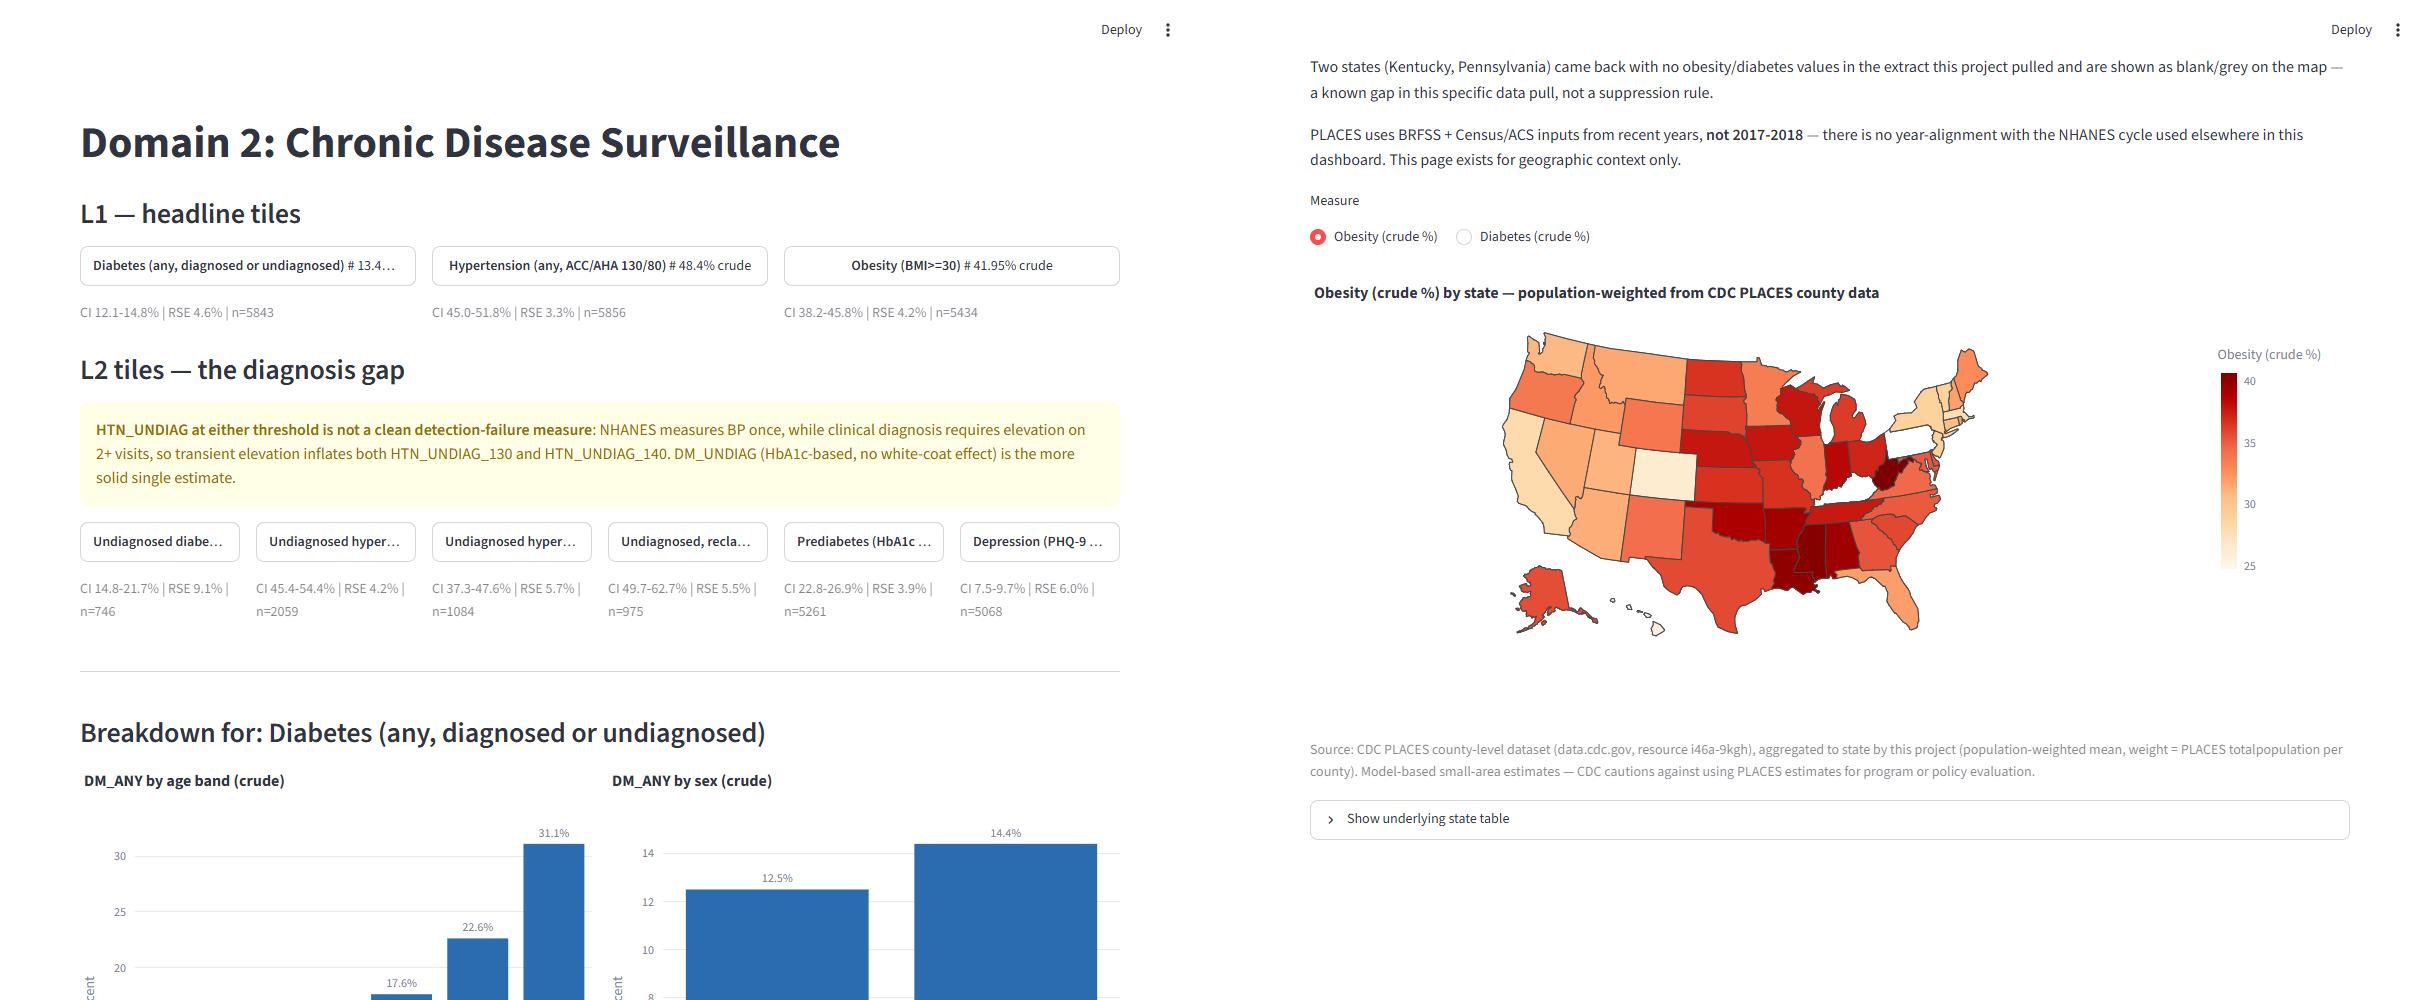
\includegraphics[width=0.64\textwidth]{figures/dashboard_pair.png}
\caption{Streamlit dashboard. Left: chronic-disease page with Level~1 headline tiles, the diagnosis-gap tiles and Level~2 breakdowns. Right: CDC PLACES state choropleth (obesity, population-weighted county estimates), labelled as a separate model-based source. Source: NHANES 2017--2018, \texttt{out/kpi\_long.csv}.}
\label{fig:dash}
\end{figure*}

\begin{figure*}[t]
\centering
\begin{minipage}{0.48\textwidth}\centering
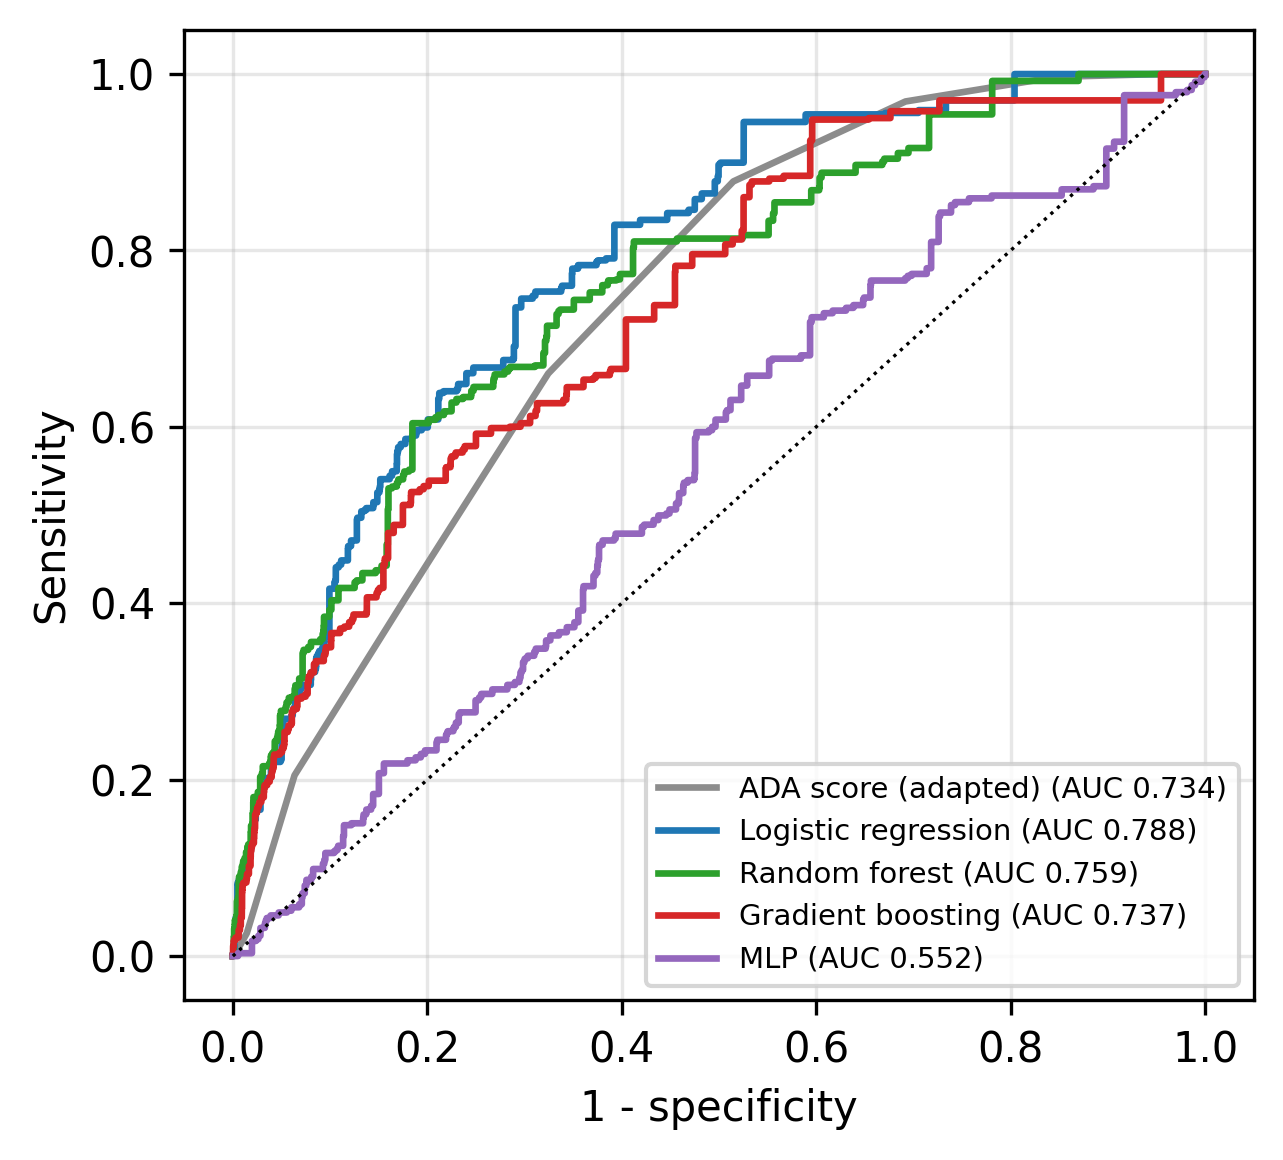
\includegraphics[width=0.72\linewidth]{figures/ml_roc.png}\\
\footnotesize (a) Weighted ROC curves, pooled out-of-fold predictions
\end{minipage}\hfill
\begin{minipage}{0.48\textwidth}\centering
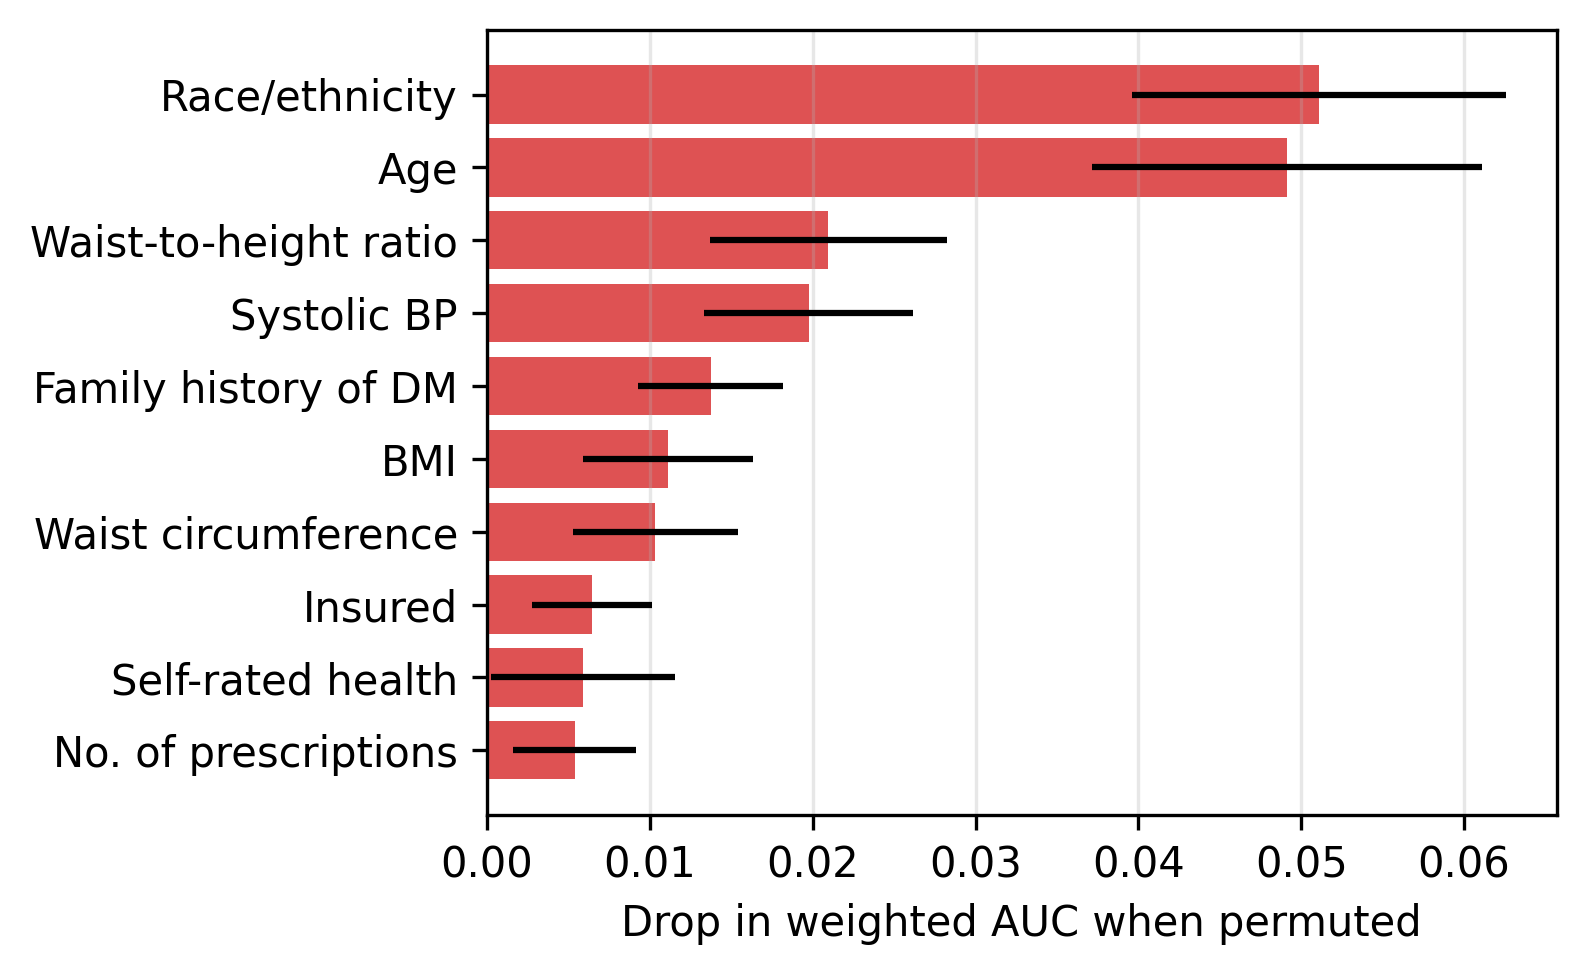
\includegraphics[width=0.86\linewidth]{figures/ml_importance.png}\\
\footnotesize (b) Permutation importance, final logistic regression
\end{minipage}
\caption{Screening results (NHANES 2017--2018, adults 20+ never told they had diabetes, MEC weights, $n=4{,}051$). Importance is the mean $\pm$ SD drop in weighted AUC over 10 permutations.}
\label{fig:roc}
\end{figure*}

\subsection{KPI estimates and the diagnosis gap}
Table~\ref{tab:kpi} gives the headline estimates. Of the 612 cells, 53 (8.7\%) were suppressed. Among adults whose HbA1c was 6.5\% or higher, an estimated 18.0\% (95\% CI 14.8--21.7, $n=746$) had never been told they had diabetes. They represent about 23.5 million adults, so roughly 4.2 million had undiagnosed diabetes. Treating ``borderline'' answers as undiagnosed gives 23.4\% (19.5--27.7), close to the 23.3\% of Wang \textit{et al.} \cite{wang2021}. Undiagnosed hypertension was 49.9\% at 130/80 and 42.4\% at 140/90, on different denominators. Both are far above the roughly 23\% unawareness of Muntner \textit{et al.} \cite{muntner2020}, because our denominator excludes treated, controlled hypertensives and blood pressure was measured at one visit. HbA1c has neither problem, so diabetes anchors the diagnosis-gap finding.

\begin{table}[t]
\caption{Headline KPI Estimates, Adults 18+, NHANES 2017--2018}
\label{tab:kpi}
\centering
\footnotesize
\setlength{\tabcolsep}{3pt}
\begin{tabular}{@{}lrrrr@{}}
\toprule
\textbf{Indicator} & \textbf{\%} & \textbf{95\% CI} & \textbf{RSE} & \textbf{$n$} \\
\midrule
\multicolumn{5}{@{}l}{\textit{Chronic disease}} \\
Any diabetes & 13.4 & 12.1--14.8 & 4.6 & 5,843 \\
Undiagnosed diabetes$^a$ & 18.0 & 14.8--21.7 & 9.1 & 746 \\
Prediabetes (HbA1c 5.7--6.4\%) & 24.8 & 22.8--26.9 & 3.9 & 5,261 \\
Hypertension (130/80 or told) & 48.4 & 45.0--51.8 & 3.3 & 5,856 \\
Undiagnosed HTN, 130/80$^a$ & 49.9 & 45.4--54.4 & 4.2 & 2,059 \\
Undiagnosed HTN, 140/90$^a$ & 42.4 & 37.3--47.6 & 5.7 & 1,084 \\
Obesity (BMI $\geq$30) & 42.0 & 38.2--45.8 & 4.2 & 5,434 \\
Depression (PHQ-9 $\geq$10) & 8.6 & 7.5--9.7 & 6.0 & 5,068 \\
\multicolumn{5}{@{}l}{\textit{Utilisation and experience}} \\
Fair/poor self-rated health & 18.6 & 16.6--20.8 & 5.3 & 5,849 \\
Admitted, past 12 months & 11.0 & 10.1--11.9 & 4.0 & 5,854 \\
$\geq$4 care contacts & 20.7 & 19.4--22.0 & 2.9 & 5,842 \\
\multicolumn{5}{@{}l}{\textit{Access}} \\
Uninsured & 13.9 & 10.3--18.5 & 13.7 & 5,837 \\
Has usual source of care & 81.2 & 78.3--83.8 & 1.6 & 5,817 \\
Polypharmacy ($\geq$5 Rx) & 16.5 & 14.5--18.7 & 6.0 & 5,856 \\
\bottomrule
\multicolumn{5}{@{}l}{\scriptsize $^a$Denominator: adults above the laboratory or measured threshold.}\\
\multicolumn{5}{@{}l}{\scriptsize Logit intervals with $t_{0.975,15}$; RSE in \%.}
\end{tabular}
\end{table}

\subsection{Income inequality}
Access and self-reported outcomes were strongly concentrated among poorer adults: uninsured $C=-0.424$ (Erreygers $E=-0.236$), fair or poor health $-0.270$ ($E=-0.201$) and depression $-0.257$ ($E=-0.088$), while undiagnosed diabetes was almost flat ($C=-0.011$) and undiagnosed hypertension was slightly concentrated among richer adults ($+0.029$ and $+0.052$). Within age bands the uninsured gradient was steeper ($-0.39$ to $-0.53$ at 30--69), so Medicare above 65 does not explain it. For any diabetes the pooled index ($-0.011$) hid a stronger gradient at 60--69 ($-0.127$), because poorer respondents are younger. Undiagnosed diabetes stayed flat in the only well-populated band ($-0.002$ at 60--69): insurance would narrow the access gap, but screening has to reach all income groups.



\subsection{Validation against published estimates}
Age-standardised obesity (41.8\%) was within one point of Hales \textit{et al.} (42.4\%, ages 20+) \cite{hales2020}. Hypertension (45.0\%) matched Ostchega \textit{et al.} (45.4\%) \cite{ostchega2020}, but their definition also counts medication users, so the match may hide offsetting differences. Any diabetes (13.5\%) was close to the national 13.2\% (12.0--14.5) \cite{cdc_ndsr} even though ours omits fasting glucose, an open question. Undiagnosed diabetes could not be standardised, as only four of eight age groups were estimable.




\subsection{Screening model performance}
The screening cohort had 4,051 adults, of whom 150 had HbA1c $\geq$6.5\% (3.7\% unweighted, 2.1\% weighted). Table~\ref{tab:ml} and Fig.~\ref{fig:roc} summarise the nested cross-validation. Logistic regression had the highest pooled out-of-fold weighted AUC, 0.788 (95\% CI 0.732--0.841), against 0.734 (0.689--0.775) for the adapted ADA score. At 80\% specificity it found 62\% of cases against 45\% for the ADA score, and its weighted AUPRC was twice as high (0.100 versus 0.048; the weighted prevalence is about 2\%). The bootstrap interval for the gain ($+0.057$, $-0.007$ to $+0.114$) includes zero, so with 150 cases the improvement is not established.

\begin{table}[t]
\caption{Nested-CV Results for Undiagnosed Diabetes (Weighted)}
\label{tab:ml}
\centering
\footnotesize
\setlength{\tabcolsep}{2.5pt}
\begin{tabular}{@{}lccccc@{}}
\toprule
\textbf{Model} & \textbf{AUC$_w$} & \textbf{Pooled AUC$_w$} & \textbf{AUPRC$_w$} & \textbf{Sens@} & \textbf{Brier$_w$} \\
 & \textbf{mean$\pm$SD} & \textbf{(95\% CI)} & & \textbf{Spec 0.8} & \\
\midrule
ADA score$^a$ & 0.734$\pm$0.014 & 0.734 (0.689--0.775) & 0.048 & 0.45 & -- \\
LR & 0.795$\pm$0.040 & \textbf{0.788} (0.732--0.841) & 0.100 & \textbf{0.62} & 0.170 \\
RF & \textbf{0.802}$\pm$0.063 & 0.759 (0.691--0.820) & \textbf{0.113} & 0.58 & 0.053 \\
GBM & 0.764$\pm$0.051 & 0.737 (0.673--0.804) & 0.094 & 0.53 & 0.073 \\
MLP$^b$ & 0.564$\pm$0.122 & 0.552 (0.474--0.628) & 0.028 & 0.21 & 0.054 \\
\bottomrule
\multicolumn{6}{@{}l}{\scriptsize $^a$Adapted, 5 of 7 items; cut-off $\geq$5 gave sensitivity 0.66, specificity 0.68.}\\
\multicolumn{6}{@{}l}{\scriptsize $^b$Unweighted (no sample-weight support). $n=4{,}051$, 150 cases, 5$\times$3 nested CV.}
\end{tabular}
\end{table}



The random forest had the best mean fold AUC (0.802) but the widest spread across folds ($\pm$0.063). Its pooled AUC was lower (0.759) because scores from five separate forests are not on a common scale. Gradient boosting picked the smaller learning rate (0.03) in every fold and trees of depth 2 or 3, and still did not beat logistic regression; with 120 training positives per fold, the extra flexibility mostly added variance. Every inner search picked the strongest regularisation for logistic regression ($C_{\mathrm{reg}}=0.01$). The MLP was close to chance: it could not use the survey or class weights, and early stopping held out a 10\% validation split containing only 8 to 12 positives. Class balancing inflated predicted probabilities (Brier 0.05--0.17), which affects calibration but not ranking.

Fig.~\ref{fig:roc}(b) ranks the inputs. Race and ethnicity and age mattered most, followed by waist-to-height ratio, systolic pressure and family history. In the standardised logistic model the odds per standard deviation were 1.74 for age, 1.46 for waist-to-height ratio and 1.39 for systolic pressure; family history multiplied the odds by 1.55, being insured by 0.69, and non-Hispanic White ethnicity by 0.50. Uninsured adults had higher odds of an undiagnosed case; fewer contacts with care is one plausible reason, though the data cannot show it.

\subsection{Comparative analysis with published models}
Table~\ref{tab:bench} compares published models. De Silva \textit{et al.} \cite{desilva2021} also targeted undiagnosed diabetes in NHANES; their ADA AUROC (0.737) is almost identical to ours (0.734), and they too found no significant ML gain. Our LR (0.788) is above their best (0.757), probably because it uses measured blood pressure and waist-to-height ratio rather than nutritional markers. AUCs above 0.85 \cite{liu2025,yang2026} come from many pooled cycles or high-risk cohorts, and \cite{qin2022,riverosperez2025} predicted fasting-glucose or self-reported diabetes, an easier target. Without survey weights, those AUCs describe the sample rather than the US population.

\begin{table}[t]
\caption{Comparison with Published Diabetes Screening Models}
\label{tab:bench}
\centering
\footnotesize
\setlength{\tabcolsep}{2.5pt}
\begin{tabular}{@{}p{1.15cm}p{2.75cm}p{1.45cm}p{1.6cm}@{}}
\toprule
\textbf{Study} & \textbf{Data, outcome} & \textbf{Model} & \textbf{AUC} \\
\midrule
\multirow{2}{*}{\cite{desilva2021} 2021} & NHANES, undiagnosed T2D & LR / RF / ANN & 0.757 / 0.752 / 0.749 \\
 & (internal) & ADA test & 0.737 \\
\cite{choi2023} 2023 & KNHANES, undiagnosed DM (external) & RF / XGB / LGBM & 0.788 / 0.802 / 0.819 \\
\cite{qin2022} 2022 & NHANES, FPG $\geq$7 mmol/L & LR / RF / CatBoost & 0.75 / 0.81 / 0.83 \\
\cite{riverosperez2025} 2025 & NHANES 2007--18, self-reported T2D & LR, RF / XGB & $\approx$0.79 / 0.817 \\
\cite{yoo2026} 2026 & NHANES, pre-DM or DM (external US) & NN, 7 inputs & 0.773 \\
\cite{liu2025} 2025 & NHANES 1999--2020, undiagnosed DM & AutoML & 0.909 \\
\cite{yang2026} 2026 & NHANES 2013--18, high-risk adults & RF / XGB & 0.896 / 0.903 \\
\midrule
\textbf{This work} & NHANES 2017--18, undiagnosed DM, \textbf{weighted} & LR / RF / GBM & 0.788 / 0.759 / 0.737 \\
 & & ADA (adapted) & 0.734 \\
\bottomrule
\end{tabular}
\end{table}

\section{Discussion and Limitations}
The estimates show that about one in five adults with laboratory-defined diabetes is undiagnosed, and unlike lack of insurance this gap is not concentrated among the poor. A small set of non-laboratory measurements ranked these cases at least as well as the ADA questionnaire, and with about 150 cases a regularised logistic model was enough.

Limitations: the data are cross-sectional (no incidence or causation); diabetes is HbA1c-only, with bias of unknown direction, so 18.0\% is not a lower bound; blood pressure is single-visit and oscillometric; the ``borderline'' answer moves the gap from 18.0\% to 23.4\%; public NHANES has no geography, and 93.6\% of uninsured variance sits in five masked strata; standardised intervals use $z=1.96$ and six or seven of eight age groups; the ML bootstrap ignores clustering. Two data errors were found and fixed: a placeholder row counted non-users of prescriptions as taking one drug, and a wrong variable name dropped COPD from the multimorbidity count.

\section{Conclusion}
This work built a three-tier KPI dashboard (Fig.~\ref{fig:dash}) whose 612 estimates carry design-based intervals and reliability flags. Undiagnosed diabetes affected 18.0\% (14.8--21.7) of adults with HbA1c $\geq$6.5\%, about 4.2 million people, and it was not graded by income, while lack of insurance was strongly concentrated among the poor ($C=-0.42$). A survey-weighted logistic regression on 18 non-laboratory inputs reached a weighted AUC of 0.788, above the adapted ADA score (0.734) but not significantly so. Next steps are to add the fasting-glucose file, pool the 2017--March 2020 and 2021--2023 cycles to increase the number of cases, and validate the model externally on the 2021--2023 data.



\bibliographystyle{IEEEtran}
\bibliography{references}

\end{document}
